\documentclass{article}
\usepackage{graphicx}
\usepackage{float}

\author{Bui Duc Anh}
\title{Installing Ubuntu 22.04.3 On VirtualBox}

\begin{document}
    \maketitle{}
    \newpage
    \section*{Downloading the ISO}
    To begin installing the Ubuntu on your Virtual Machine, we must first download the ISO from Ubuntu's website.
        \begin{figure}[H]
            \centering
            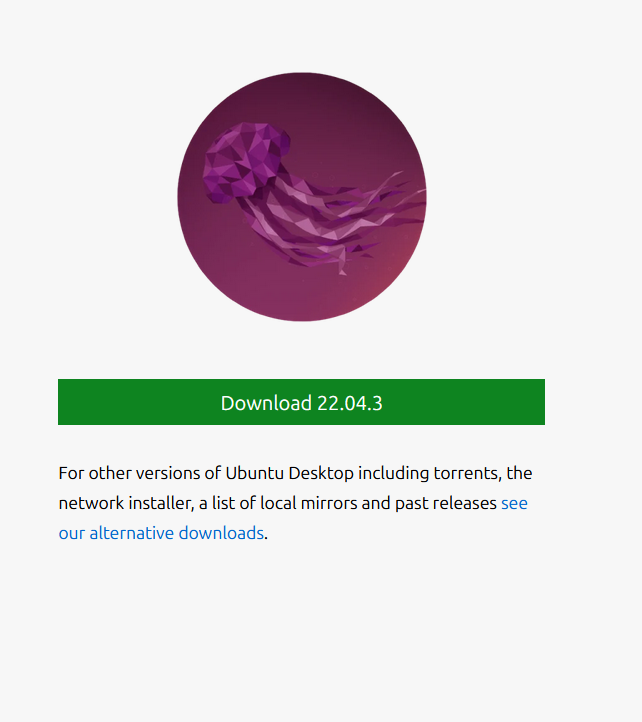
\includegraphics{Pics/Download_Page.png}
            \caption{Download Ubuntu 22.04.3 ISO}
            \label{fig:Going to the website}
        \end{figure}
    \section*{Installing the ISO}
    \subsection*{Opening VirtualBox}
    Once you've got your ISO downloaded, We must open VirtualBox then click on "New"
    \begin{figure}[H]
            \centering
            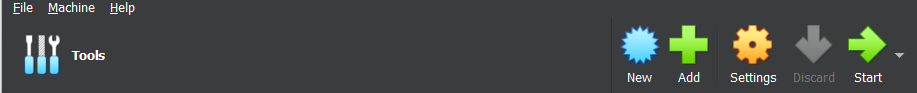
\includegraphics{Pics/New_Example.png}
            \caption{New Button}
        \end{figure}
    \subsection*{Creating The VM}
    Then once you're in the New window, choose the name for your Virtual machine and select the Ubuntu ISO we just downloaded, then continue.
    \begin{figure}[H]
        \centering
        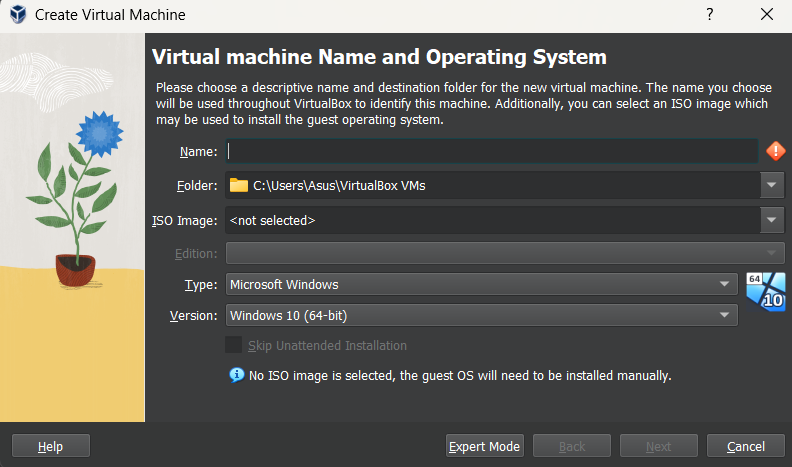
\includegraphics{Pics/New_Window.png}
        \caption{New Window}
    \end{figure}
    \subsection*{Choosing your username and password}
    \begin{figure}[H]
        \centering
        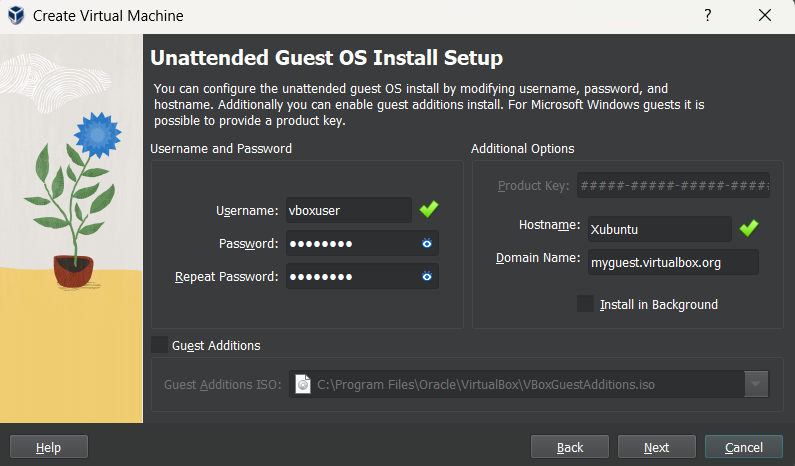
\includegraphics{Pics/Next_1.png}
        \caption{Password and Username}
    \end{figure}
    \subsection*{Hardware modifications}
    Some advice for choosing Hardware options for the VM
    \begin{itemize}
        \item Memory (RAM): Ubuntu Desktop typically requires at least 2 GB of RAM for basic functionality. If you plan to run more resource-intensive applications or multiple applications simultaneously, consider allocating more RAM. For development or multitasking, 4 GB or more is often recommended.
        \item Processor (CPU): Ubuntu can run on a wide range of processors, but a multi-core processor will provide better performance, especially if you're running resource-intensive tasks. A dual-core or quad-core processor is often sufficient for most general purposes.
        \item Storage: The disk space required for Ubuntu depends on the installation type and the applications you plan to install. A minimal installation might need around 25 GB, but for a more comfortable experience, especially if you intend to install additional software, 50 GB or more is recommended. Consider using an SSD for improved performance.
    \end{itemize}
    \begin{figure}[H]
        \centering
        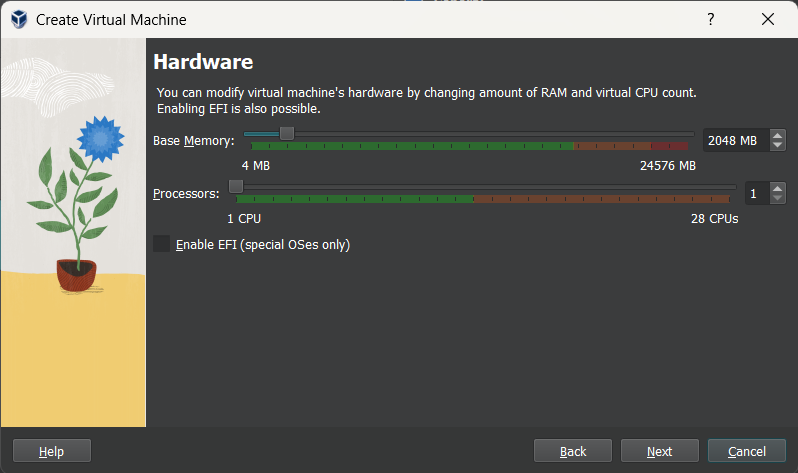
\includegraphics{Pics/Hardware_Modification_Window.png}
        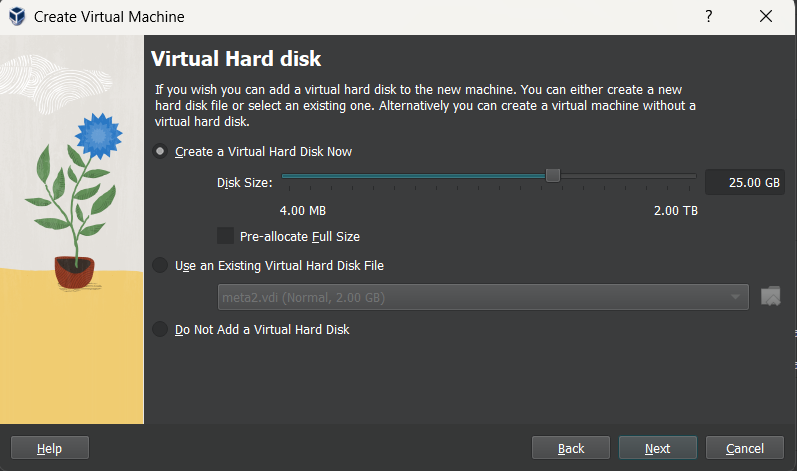
\includegraphics{Pics/Hardware_Modification_Window_Next.png}
        \caption{Hardware}
    \end{figure}
    \section*{Finishing}
    Congratulations after pressing next all the way you have finished installing Ubuntu on your VirtualBox. Now all that is left is to boot it up and wait for it to install all the required components.
\end{document}